\title{Initial Report on Raytracing}
\author{Team Raytrashing}
\date{February 2018}

\maketitle

\section{Aims}
Our main aim as a team is to implement a working Raytracer with an efficient back-end coupled with a savvy front-end. We also intend to learn new software, technologies and tools (like Python, JavaScript, TravisCI etc.) as a part of this project and we want to do so by working together as a team. 
As far as the specific technical aims of the project are concerned, we wish to implement a raytracer with the following features and their priorities/levels given in the brackets (1 being the highest priority on a scale of 10):
\begin{itemize}
    \item Translucency (1)
    \item Shadows (1)
    \item Reflection (1)
    \item Rendering multiple shapes like sphere, cube, pyramid etc. (1)
    \item Ability to render the shapes within 30-40 seconds (1)
    \item Responsiveness on the front-end (2)
    \item Client-Server Architecture (2)
    \item Distributed Systems and Multi-Threading for faster performance (2)
    \item Drag and Drop capability on the front-end (2)
    \item Making the website secure - HTTPS (3)
    \item Ability to change the camera position (3)
    \item Saving the current scene for future reference (4)
    \item Live-rendering using thumbnails (4)
\end{itemize}
We wish to implement these by continuously referring to the milestone plan by keeping in mind the priorities of each task.


\section{Strategy}
Our team convened to discuss which technologies to use for the Raytracer implementation and during the first meeting, we had decided to use Python and Django for the back-end and JavaScript coupled with HTML and CSS for the front-end. The reason to choose Python and JavaScript for the development was because none of us had previously extensively worked on either of the technologies and we thought this is a good opportunity to learn and hone our skills in these languages. \par
Our strategy is also to reduce the number of bugs we have to deal with and hence we have accepted that our development will follow Test Driven Development (TDD) and Pair Programming. We are following TDD by creating test cases and then developing so that we can reduce the number of bugs. Pair programming also helps in avoiding buggy code. \par
As a team, we also decided that we would be using the Agile methodology for our software development. We are following weekly Sprint cycle and we convene on Tuesdays from 1300 Hrs to 1600 Hrs by booking a room with the help of King's Venues.
We use Trello boards for maintaining the tasks and keeping track of them and during the weekly meetings, we accept previous sprint's tasks and define new tasks for the upcoming sprint.\par
Initially, we did face some problems with the communication among the team members. Some minor confusion ensued in the first week but everything got back on track after everyone got accustomed with the tools and the technologies. We, as a team, got familiar with GitHub and the nuances of it like feature branches and pull requests. We have put in a lot of effort till now and just within two weeks of the start of the group project we have a working front-end and back-end and we are ready with the prototype. We are on track with what we set as milestones in the milestone plan and the aims of the project.

\begin{figure}[htb]
\centering
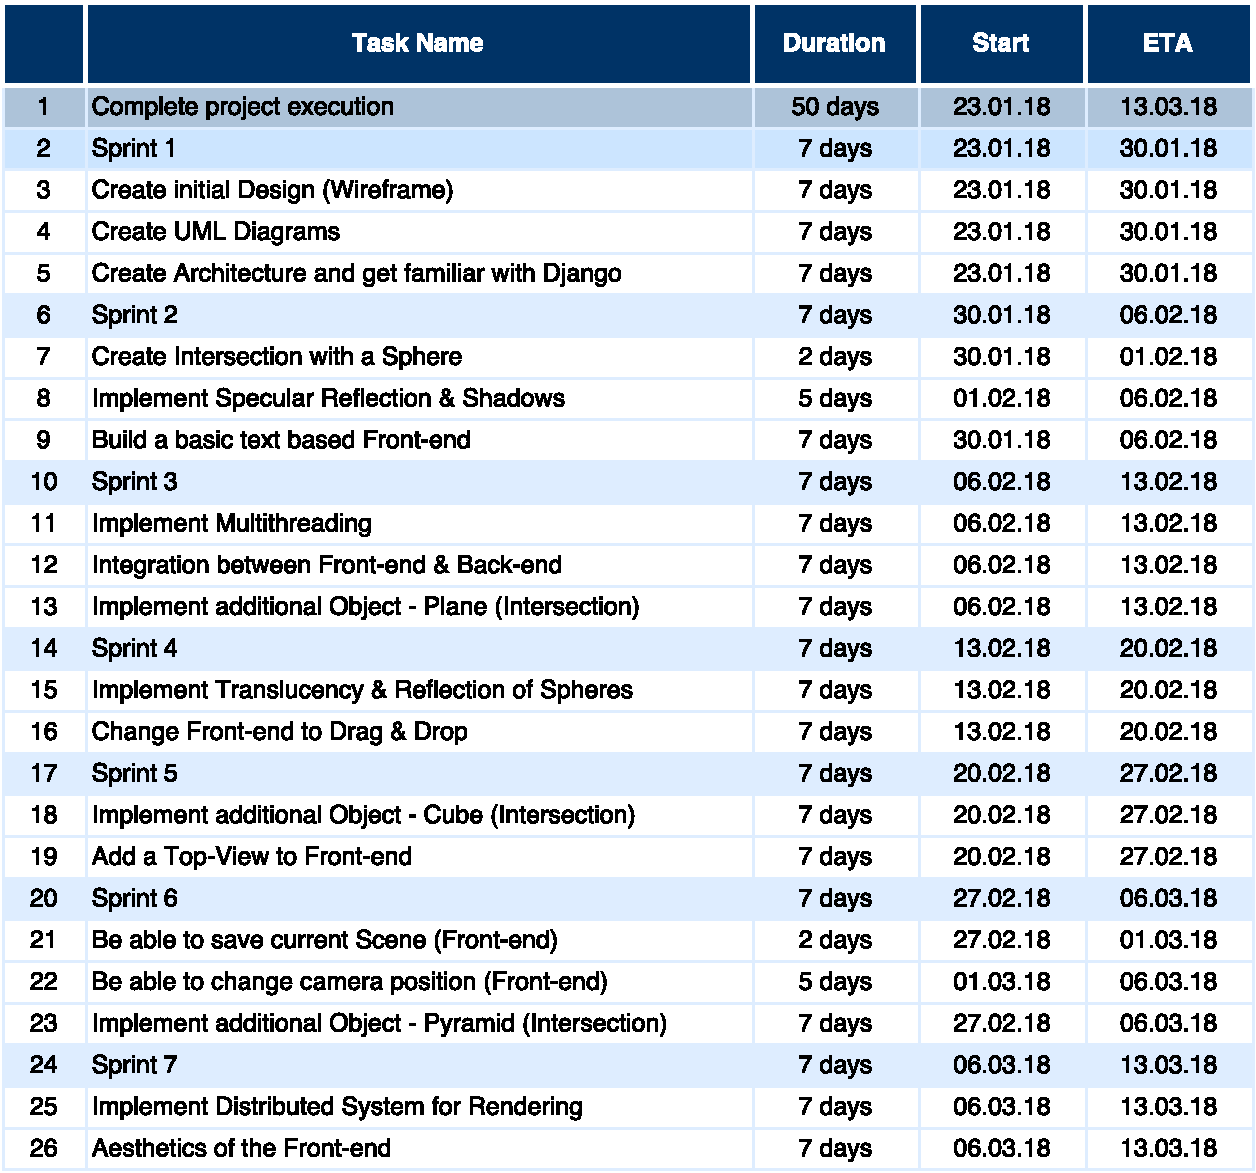
\includegraphics[width=0.8\textwidth]{images/time_table.pdf} % To change the image size, change the factor 0.8
\caption{Project Time Table} 
\label{fig:TimeTable} 
\end{figure}